%\textbf{background - why do merging clusters of
%galaxies are worthy of investigating}
%Clusters of galaxies are some of the most interesting astrophysical
%laboratories. The environment of the cluster affects the evolution of the
%galaxy members. Redder galaxies are located closer to the dynamical
%centers of galaxies while bluer star-forming galaxies are located at the
%edge of clusters.

%----------------------------------------------------------------------
% To do:
% - make sure that when introduce the 2 subclusters - talk about the 
%   NW and SE notation
% - add Williamson 's paper as one of the reference for the first mention
%   of El Gordo
%----------------------------------------------------------------------

%\textbf{to motivate why we want to do this study} 
\textbf{Mergers of dark-matter-dominated galaxy clusters probes properties
of the cluster components like no other systems}. 
Clusters of galaxies are made up of 80\% of dark matter in mass content, 
with a smaller  portion of intercluster gas($\sim 15\%$ in mass content), and
sparsely spaced galaxies ($\sim 2\%$ in mass content) (REF). During a merger of
clusters, the subclusters are accelerated to high speeds of several
thousand \kilo \meter~\second$^{-1}$. The offsets of different components
of the subclusters dissociate show how various interactions of the different
components are at work. Observables such as offset between dark
matter and the other components may suggest dark matter self-interaction
(REF).  The difference of the galaxy colors in a merging cluster from relaxed cluster can also verify effects of environment on galaxy evolution.\par
%\textbf{background of El Gordo}
%\textbf{What literature exists for El Gordo.}

\textbf{Ever since the discovery of El Gordo in the Atacama Camera Telescope (ACT)
survey (REF), there is an ongoing effort for collecting comprehensive data
for El Gordo.} From the spectroscopy and Dressler-Schecter test for the member galaxies  in Sif\'{o}n et al. (2013), El Gordo is confirmed to be a binary merger 
without significant substructures. This picture is further supported by the
weak lensing analysis by Jee et al. (2013). The weak lensing analysis shows
a mass ratio of 2:1  between the two main subclusters, named according to their location as the northeast (NW) and southeast (SE) subclusters respectively. 
(See Figure \ref{fig:config}). El Gordo has interesting intracluster medium morphology as shown in the X-ray. In the northwest, it shows a wake feature, i.e.,
depression in the X-ray emissivity, while in the southeast, it shows
highest X-ray emissivity indicative of a cold gas core southeast of the
wake. The cold gas core may have passed from the northwest to the southwest
to have caused this morphology (Menanteau et al. 2011, hereafter M11). 
The extended mass distribution of El Gordo also makes it a good
gravitational lens. Zitrin et al. (2013) have found multiple strong
gravitationally lensed images around the center region of El Gordo. 
On the outer skirt of El Gordo, strong radio emission is detected in
the NW and the SE respectively. These radio emission has steep spectral
index gradient and are identified as radio relic created from a merger.\par 
%\begin{itemize}
%\item explains the 2D configuration of El Gordo - bimodal
%\item evidence that it is a merger 
%goes along a line joining northwest to southeast. 
%\item explains the spectroscopic surveys which confirms that that there are
%not a lot of line of sight substructures and that the line-of-sight
%velocity difference of the  
%\item strong lensing - many many arcs and elongated lens weak-lensing -
%bimodal distribution of matter  (describes what data has been available for 
%El Gordo) Since the
%discovery, an abundance of multi-wavelength data of El Gordo has been
%analyzed according to the two-dimensional projected view. \par 
%\item explain the wake feature (depression in X-ray) and the cold core in
%the SE which has high X-ray emission and point out it shows a recent merger 
%unlike the bullet cluster, El Gordo lacks a prominent X-ray shock
%\end{itemize}\par
%\textbf{Explains the importance of radio relic in constraining the merger
%physics.} Radio relics are direct products of the merger process itself.
%
%\begin{itemize}
%
%\item explains the double radio relic and their formation
%synchrontron emission in the radio wavelength with steep falloff of
%spectral indices.
%\item explains compression of magnetic field would cause polarization
%signal perpendicular to the merger axis 
%\item explains the current status of simulations in understanding radio
%relic
%\item  
%\end{itemize}
\begin{figure}
	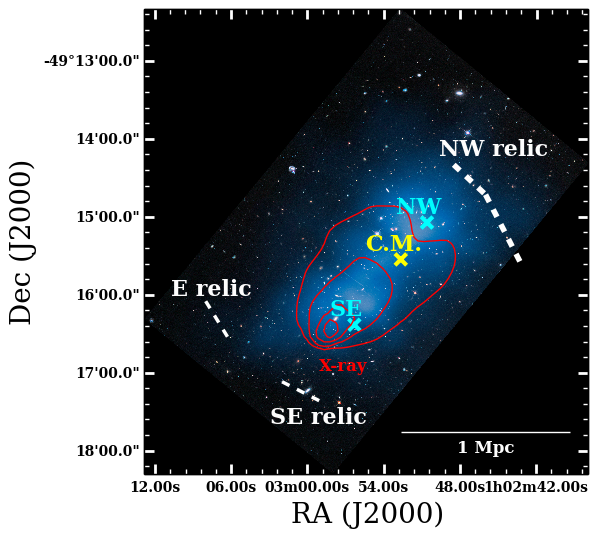
\includegraphics[width=\linewidth]{ElGordo.png}
	\caption{Configuration of El Gordo (to decide which figure to use,
	this one is from Lindner et al.) \label{fig:config}}
\end{figure}
\textbf{El Gordo is one of small sample of galaxy clusters ($\sim 50$) that have
been associated with a radio relic. (This paragraph needs a lot more
organization)} Even fewer of them have been studied in
great details, making El Gordo a valuable candidate for further analysis. 
%Cosmological simulations have largely complement the studies of the
%observed radio relics.  
%The study of radio relics is just taking off. 
%Cosmological
%simulations have also been employed to study the properties of the radio
%relics. (explain how both observations and simulations confirm radio relics
%are due to a cluster merger and that double relics are proposed to
%correspond to binary mergers)
%Radio relic, also known as radio shockwaves, are created during the violent
%merger of clusters of galaxies (See Ensslin's paper for a review of the
%physics). 
%Such double radio relics are also exhibited in other confirmed merging clusters of galaxies, such as REF missing etc. 
%
%(more description of how the paper comes up with emission in their simulations)
%
%\textbf{(Need to add transition from background to this paragraph to
%motivate why we have to study El Gordo) 
Furthermore, El Gordo satisfies the four criteria for being a dissociative merger which are proposed to be excellent
probes of self-interacting dark matter (Dawson et al. 2012) . (1) The subclusters
of El Gordo has a small ratio of mass, i.e. $\sim 2:1$ (Jee et al. 2013,
hereafter J13). (2) The merger axis, the line joining the two subclusters,
coincides with the alignment of the double radio relic propagating outward at the periphery of the cluster (Menauteau et al. 2012,
hereafter M12). This suggests a simple merger configuration with small
impact variables.  (3) The X-ray luminosity peak is shown to be offset
from the weak-lensing peak by X kpc at X $\sigma$ level (J13). (4) The
observation of the double radio relic suggests that the angle between the
merger axis and the plane of the sky has to be reasonably small (M11,
Lindner et al. 2013), or else
the relic may appear as a halo instead. \citep{S13} \par 


%\textbf{motivation} 
%\textbf{summarizes what is missing for the understanding of the merger of El
%Gordo, which is the projection angle and the time-since-collision.}
\textbf{In this paper, we perform results of simulations for modeling the time
evolution of the mergers.} 
Determining the time-since-collision of mergers of similar clusters helps
us reconstruct different stages of a cluster merger.
Mergers of clusters proceed on the time-scale of millions of year,
observations of each cluster only provides a snapshot of a particular type
of merger. In order to understand the merger process observationally, 
we need to capture
and identify different stages of similar dissociative mergers. \par 

\textbf{Another crucial piece of missing information is the 3D
configuration, i.e. the projection angle $\alpha$, which contributes the
largest amount of uncertainties to the dynamical variables (\citep{D13}).}
With a large projection angle $\alpha$, the radio emission may appear as a
radio halo instead.  \citep{S13}\par 
%\textbf{motivation2}
\textbf{This work is particularly important since it is forbiddingly
expensive to simulate clusters similar to El Gordo in high resolution. 
The probability for finding an analog of El Gordo in a cosmological
simulation is as low as \% (REF)}. A realistic cosmological simulation of
El Gordo is thus computationally expensive. Under the hierarchical picture
of structure formation in the $\Lambda$CDM model, there is a rare
chance for massive clusters like El Gordo to have formed at a redshift of
$z = 0.87$.  Staged simulation would not be able to probe the angular
dependence. 
Both weak lensing analysis and BLAH DATA of El Gordo (\citep{Jee13}) has revealed a
relatively simple bimodal mass distribution.  The lack of complex
substructures makes modeling of El Gordo with only two subclusters possible.

\par

\textbf{In this paper, we adopt the following conventions:} (1) we
assume the standard $\Lambda$CDM cosmology with $\Omega_{m} = 0.3$, $\Omega_{\Lambda} = 0.7$. (2) All confidence intervals are quoted at the 68\% level unless otherwise stated. 
(3) All credible intervals (a.k.a. Bayesian confidence intervals) are also
quoted at the 68\% level unless otherwise stated and are central credible
intervals. (4) All quoted masses ($M_{200c}$) are based on mass contained
within $r_{200}$ where the mass density is 200 times the critical density
of the universe ($\rho_{crit}$) at the redshift of $z = 0.87$. 
%(5) We
%demonstrate that the application of a uniform sampling PDFs derived due to the
%integrated polarization fraction of the radio relic does not introduce
%large biases into our estimators in section \ref{sec:relic}, and unless
%otherwise stated, the simulation results we quote are those after applying
%the uniform radio relic filter.  \par 
